% MCDS Capstone Final Report
% Kyle Dotterrer
% 21 November, 2021

%% ==================================================================
%% BOILERPLATE
%% ==================================================================

\documentclass{vldb}

\newcommand{\paperTitle}{JIT Compilation for User-Defined Functions\\ 
    \large MCDS Capstone Final Report\\
    \today}
\newcommand{\paperKeywords}{}
\newcommand{\paperAuthors}{}

\setlength{\paperheight}{11in}
\setlength{\paperwidth}{8.5in}

\usepackage[
            bookmarks=true,
            bookmarksopen=true,
            pdfhighlight=/I,
            pdfpagemode=UseOutlines,
            linkcolor=blue,
            pdfborder={ 0 0 0 },
            pageanchor=false]{hyperref}
\hypersetup{
    pdfauthor = {\paperAuthors},
    pdftitle = {\paperTitle},
    pdfkeywords = {\paperKeywords},
    pdfborder={ 0 0 0 }
}

\usepackage{amsmath}
\usepackage{amssymb}
\usepackage{times}
\usepackage{boxedminipage}
\usepackage{xspace}
\usepackage{array}
\usepackage{epsfig}
\usepackage{calc}
\usepackage{multirow}
\usepackage{rotating}
\usepackage{enumitem}
\usepackage[usenames,dvipsnames]{color}
\usepackage{tabularx}
\usepackage{tikz}
\usepackage{wasysym }
\usepackage[hyphenbreaks]{breakurl}
\usepackage{xcolor}
\usepackage[font={small}]{caption}
\usepackage{alltt}
\usepackage{setspace}
\usepackage{wrapfig}
\usepackage{etoolbox}
\usepackage{enumitem}

% Font selection
\usepackage[final]{microtype}
\usepackage[scaled]{inconsolata}
\usepackage[T1]{fontenc}
\usepackage{graphicx}
\usepackage{soul}
\usepackage{pifont}

% Other misc. things
\usepackage{float}
\usepackage{bookmark}
\usepackage{amsmath,amsfonts,amssymb}
\usepackage{latexsym}
\usepackage{multirow}
\usepackage{emptypage}
\usepackage{booktabs}
\usepackage{braket}
\usepackage{balance}

\usepackage[newfloat]{minted}

\definecolor{commentgray}{rgb}{0.2,0.2,0.2}
\definecolor{bggray}{rgb}{0.98,0.98,0.98}

\setminted{
  bgcolor=white,
  numberblanklines=false,
  frame=single,
  numbers=left,
  tabsize=2,
  xleftmargin=1.8em,
  xrightmargin=0.5em
}


%% ==================================================================
%% MACROS
%% ==================================================================

\newcommand{\subparagraph}{}

\newcommand{\sysname}{NoisePage\xspace}

% Framework Components
\newcommand{\dbTranslator}{Translator\xspace}
\newcommand{\dbCompiler}{Compiler\xspace}
\newcommand{\dbPlanner}{planner\xspace}
\newcommand{\dbInterpreter}{interpreter\xspace}
\newcommand{\dbAnalyzer}{analyzer\xspace}
\newcommand{\dbPCQ}{PCQ\xspace}
\newcommand{\dbAQP}{AQP\xspace}
\newcommand{\dbHook}{hook\xspace}
\newcommand{\dbHooks}{hooks\xspace}

\newcommand{\dbSQL}[1]{\texttt{\textbf{#1}}\xspace}
\newcommand{\dbTable}[1]{\texttt{\MakeUppercase{#1}}\xspace}
\newcommand{\dbColumn}[1]{\texttt{col#1}\xspace}
\newcommand{\dbRawColumn}[1]{\texttt{#1}\xspace}
\newcommand{\dbConfig}[1]{\textsf{#1}\xspace}

\newcommand{\dbmsOracle}{Oracle\xspace}
\newcommand{\dbmsDBTwo}{DB2\xspace}
\newcommand{\dbmsTeradata}{Teradata\xspace}
\newcommand{\dbmsHANA}{HANA\xspace}
\newcommand{\dbmsMSSQL}{SQL Server\xspace}
\newcommand{\dbmsMySQL}{MySQL\xspace}
\newcommand{\dbmsPostgres}{PostgreSQL\xspace}
\newcommand{\dbmsMemSQL}{MemSQL\xspace}
\newcommand{\dbmsHyper}{HyPer\xspace}
\newcommand{\dbmsVector}{Vector\xspace}

\newcommand{\tplType}[1]{\texttt{#1}\xspace}
\newcommand{\tpl}{\texttt{TPL}\xspace}
\newcommand{\tbc}{\texttt{TBC}\xspace}
\newcommand{\dbCode}[1]{{\sffamily\small \textbf{#1}}\xspace}

\newcommand{\tidlist}{\texttt{TupleIdList}\xspace}
\newcommand{\tidlists}{\texttt{TupleIdLists}\xspace}

%% ==================================================================
%% PAPER CONTENT
%% ==================================================================

\begin{document}

\title{\paperTitle}

\numberofauthors{2}
\author{
    \alignauthor Kyle Dotterrer, Andrew Pavlo\\
    \affaddr{Carnegie Mellon University}\\
    \email 
        \{\href{mailto:kdottere@cs.cmu.edu}{kdottere},
        \href{mailto:pavlo@cs.cmu.edu}{pavlo}\}@cs.cmu.edu\\
}

% Remove the space for the copyright box for VLDB
\makeatletter
\def\@copyrightspace{\relax}
\makeatother

\maketitle

%% ==================================================================
%% ABSTRACT
%% ==================================================================

\section*{Abstract}

User-defined functions (UDFs) are a powerful tool for expressing complex application logic in SQL queries. Although they offer a practical complement to SQL, their use in production database environments is often limited because of their associated performance costs \cite{froid, apfel}. In this project, we evaluate the efficacy of methods intended to address the performance limitations of UDFs in the context of database management systems (DBMSs). We compare the performance of an existing, state-of-the-art technique, UDF inlining, with our own novel strategy that executes UDFs as native code via JIT-compilation. In an experimental evaluation, we find that UDF JIT-compilation and UDF inlining provide similar levels of performance benefits.

%% ==================================================================
%% INTRODUCTION
%% ==================================================================

\section{Introduction}

User-defined functions (UDFs) are a powerful tool for encapsulating complex application logic that may subsequently be embedded into SQL queries. Consider a scenario in which we would like to write a query that computes the "reward level" for each customer in a table of retail transactions based on the total amount spent by each customer. Expressing such a query in pure SQL is certainly possible, but non-trivial. In contrast, with the help of SQL's procedural extensions, the definition of a UDF that implements this logic is straightforward, as shown in figure~\ref{fig:cust_level_def}.

\begin{listing}[H]
    \begin{minted}[frame=lines]{plpgsql}
CREATE FUNCTION cust_level(ckey int)
    RETURNS CHAR(10) AS $$
    DECLARE total FLOAT;
    DECLARE level CHAR(10);
BEGIN
    total = (SELECT SUM(o_totalprice) 
        FROM orders WHERE o_custkey=ckey);
    IF (total > 1000000)
        level = 'Platinum';
    ELSE
        level = 'Regular';
    END IF;
    RETURN level;
END 
$$ LANGUAGE PLPGSQL;
    \end{minted}
    \caption{The definition of UDF \dbCode{cust\_level}.}
    \label{fig:cust_level_def}
\end{listing}

Once the UDF is defined, we can then use the UDF in subsequent queries to efficiently express high-level application logic. A query that invokes the UDF \dbCode{cust\_level} is shown in figure~\ref{fig:cust_level_call}.
    
\begin{listing}[H]
    \begin{minted}[frame=lines]{plpgsql}
SELECT c_custkey, cust_level(c_custkey)
    FROM customer;
    \end{minted}
    \caption{The invocation of UDF \dbCode{cust\_level}.}
    \label{fig:cust_level_call}
\end{listing}

This simple example demonstrates the power of user-defined functions. UDFs allow us express SQL queries more efficiently and in a manner that encourages modularization and reuse. However, UDFs present one major limitation that often precludes their use in production systems: they introduce an intolerable amount of runtime overhead. One study from Microsoft Research found that introducing UDFs to express portions of query logic can increase total execution time by over 46,000x its baseline value when expressed in pure SQL \cite{froid}. The underlying reason for this massive performance degradation is the fundamental mismatch between declarative SQL and the imperative language of UDFs. Because the source languages are so different, most database systems rely on a distinct subsystem to implement UDF execution, and the context switching between these subsystems combined with the lack of optimization applied within the UDF engine produces this impressively-poor performance \cite{froid, apfel}.

Various approaches to addressing this problem have been proposed. The most promising existing strategies for improving UDF execution performance may be approximately grouped under the term \textit{UDF inlining}. In UDF inlining, the imperative code that implements the UDF is translated to SQL, and the resulting SQL is then inserted into the calling query at the invocation site of the UDF. In this project, we propose a new approach to UDF execution that operates by leveraging an existing code generation system to JIT compile the UDF to native machine code and subsequently execute it. We implement this technique in the NoisePage \cite{noisepage} DBMS.

The remainder of this document is structured as follows. In Section 2 we provide background on query compilation and UDF compilation for analytics. In Section 3 we survey related work on UDF runtime optimization, focusing on approaches to UDF inlining. In Section 4 we describe the architecture of the query execution engine in NoisePage and in Section 5 we describe our extensions to support UDF compilation. Section 6 presents the results of our experimental evaluation. We discuss directions for future work in Section 7 and conclude in Section 8.

%% ==================================================================
%% BACKGROUND
%% ==================================================================

\section{Background}

In this section, we provide general background on the technical concepts relevant to our project. The two topics of interest include query compilation in the context of database management systems and UDF compilation in distributed analytics frameworks.

\subsection{Query Compilation}

In traditional disk-oriented systems, the DBMS implements query execution entirely in software. The canonical execution strategy employed by many database systems begins as the optimizer converts the abstract syntax tree produced by parsing the query text into a physical plan tree. Each node in this plan tree represents a physical operator that implements one or more logical operations specified in the input query, such as a \dbCode{SELECT} operation, application of a filter (\dbCode{WHERE}), or a \dbCode{JOIN}. With the plan tree constructed, the DBMS executes the query by evaluating each operator in the physical plan \cite{graefe93, graefe94, dbconcepts}. 

In this strategy, the DBMS implements its execution engine in terms of high-level, general-purpose code. This degree of generality is excellent from a software engineering perspective because it makes query execution easy to reason about. However, this comprehensibility comes at the cost of runtime performance. The generality of the code in this execution technique imposes runtime overhead by way of the many levels of indirection that it introduces, resulting in a large number of native instructions being executed \cite{freedman14}. The number of executed instructions is often not a limiting factor in disk-oriented systems' performance because disk IO operations dominate the total query processing time. For in-memory systems where persistent storage no longer imposes this bottleneck, several strategies are available to reduce the number of instructions executed in query processing.

Query compilation is one such query execution strategy that is growing in popularity. At a high level, query compilation aims to reduce the number of instructions executed by generating specialized code for each query that the system encounters. 

There are many approaches to implementing query compilation, and the techniques for doing so have evolved rapidly in the last decade. One of the earliest implementations of query compilation in the modern era was accomplished by the HIQUE system \cite{systemr}. In HIQUE, the execution engine first translates an input query to C++ code. It subsequently compiles this C++ code to native code by spawning an external process (GCC \cite{gcc}) \cite{krikellas10}. It is important to note here, however, that HIQUE does not implement translation for arbitrary SQL queries but instead relies on pre-defined C++ templates that it applies to a limited subset of input queries.

More advanced systems eschew using an external compiler to avoid the high costs associated with compilation under this model. Spawning an external compilation process introduces the latency associated with operating system process management into the critical path of query execution. Furthermore, utilizing an external compiler like GCC to compile specialized query code discards much of the information that the DBMS has already `learned' about the query while constructing its query plan and forces the compiler's frontend to repeat much of this work. The HyPer main memory DBMS \cite{hyper} is one example of a system that avoids these issues by implementing query compilation without using an external compiler. HyPer generates LLVM \cite{llvm} intermediate representation from the input query and subsequently utilizes the existing LLVM infrastructure to JIT-compile the IR to native machine code that implements the query \cite{neumann11, kemper11}.

The SingleStore \cite{singlestore} execution engine represents a more advanced approach to compilation. It first translates SQL queries to an internal domain-specific language (DSL) that then undergoes a second stage of translation to LLVM intermediate representation. The execution engine then JIT-compiles this intermediate representation to native code \cite{paroski16}. This additional step in the query compilation process facilitates greater developer productivity by making it easier to reason about the code generated by the execution engine's upper layers.

Carnegie Mellon Database Group's NoisePage system implements an approach to query compilation that is similar to SingleStore's. The first step in NoisePage's query processing pipeline is translation of the input query to an internal domain-specific language. The execution engine then compiles this DSL to a lower-level bytecode representation. Once this bytecode is generated, the NoisePage execution engine can either run the bytecode directly on an interpreter or translate this bytecode to LLVM IR that is then JIT-compiled to efficient machine code \cite{pcq}.

\subsection{UDF Compilation for Analytics}

Outside of the database systems community, the term ``user-defined function'' has a more general definition. In general analytical applications, a user-defined function is any functionality that is not built into the processing engine itself, and is instead written by an end-user.

%% ==================================================================
%% RELATED WORK
%% ==================================================================

\section{Related Work}

In this section, we describe approaches to UDF runtime optimization. These approaches are relevant for our discussion because they are the baseline against which we measure the effectiveness of our approach.

Tradition DBMS execution engines are not equipped to execute arbitrary imperative program logic. For this reason, many systems implement a distinct execution subsystem for procedural extensions to SQL and perform a context-switch from the primary SQL execution engine to this subsystem whenever a UDF must be evaluated \cite{apfel}. An example of this style of UDF evaluation is shown in figure~\ref{fig:overhead_simple}.

\begin{figure}[t!]
    \centering
    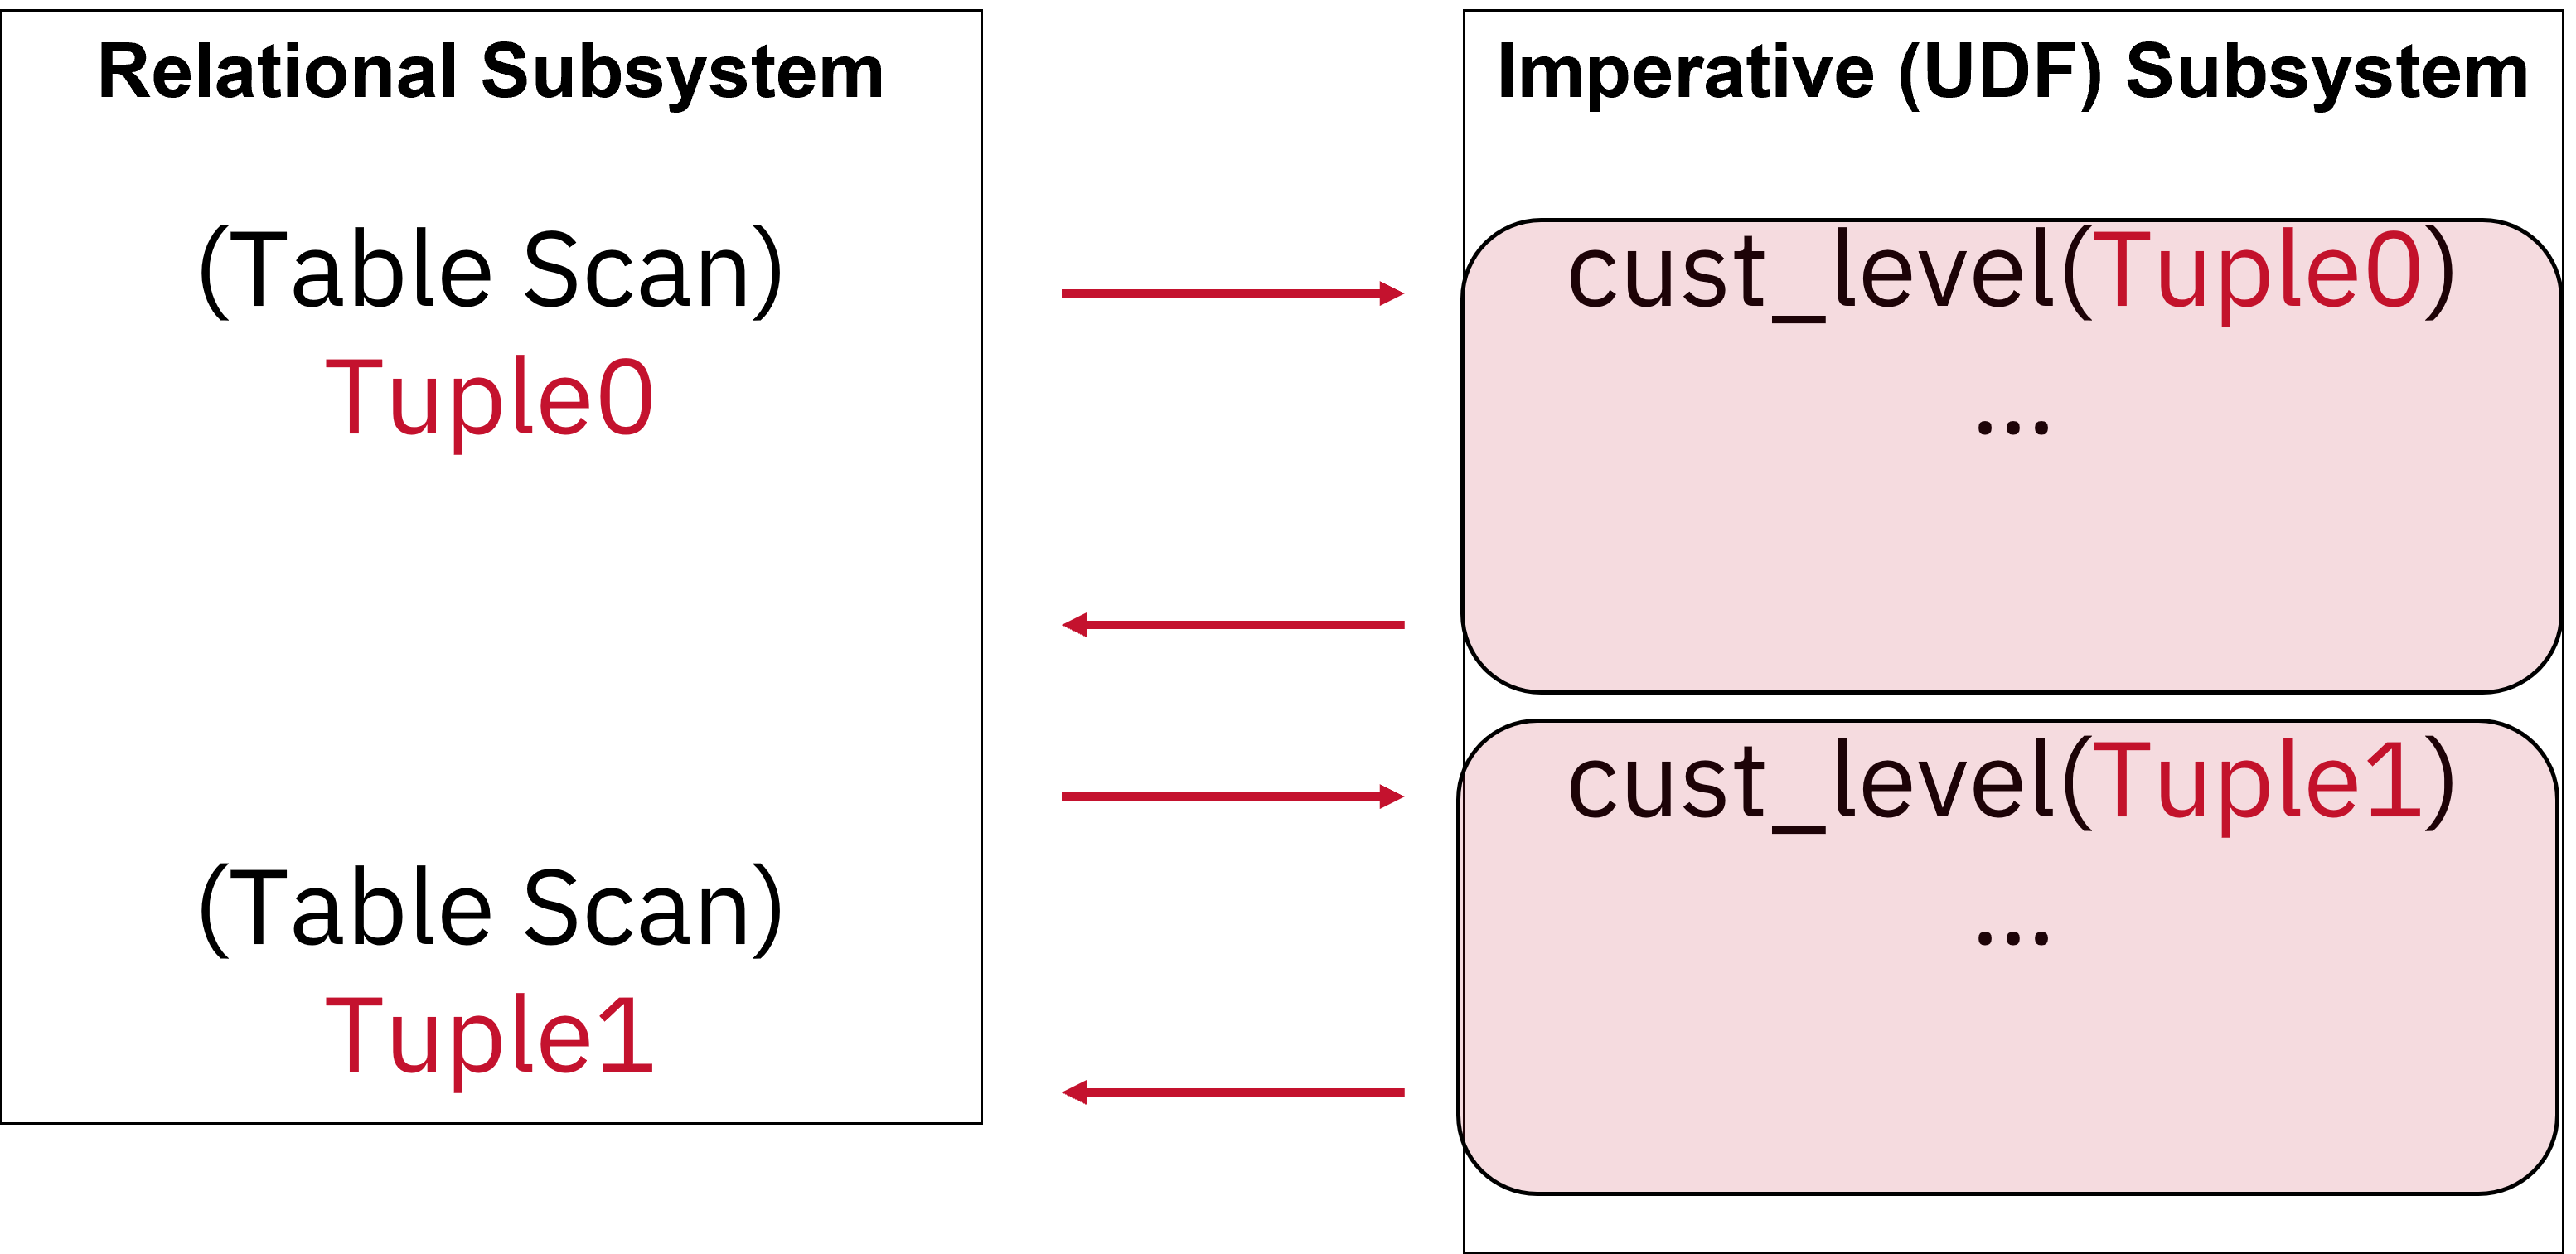
\includegraphics[width=\columnwidth]{img/overhead1.png}
    \caption{
        \textbf{Interpreted UDF Execution} --
        In a traditional DBMS execution engine, the SQL execution engine must context switch to a distinct execution engine for imperative code whenever it encounters a UDF.
    }
    \label{fig:overhead_simple}
\end{figure}

While this approach makes combining the two styles of execution simple to reason about, it often implies significant performance penalties. Frequent context-switching between the SQL engine and the imperative subsystem imposes huge runtime overhead. The situation is made worse by the fact that most UDFs contain embedded SQL queries, leading to further context-switches from the UDF subsystem back to the SQL engine. An example of this situation is shown in figure~\ref{fig:overhead_complex}.

\begin{figure}[t!]
    \centering
    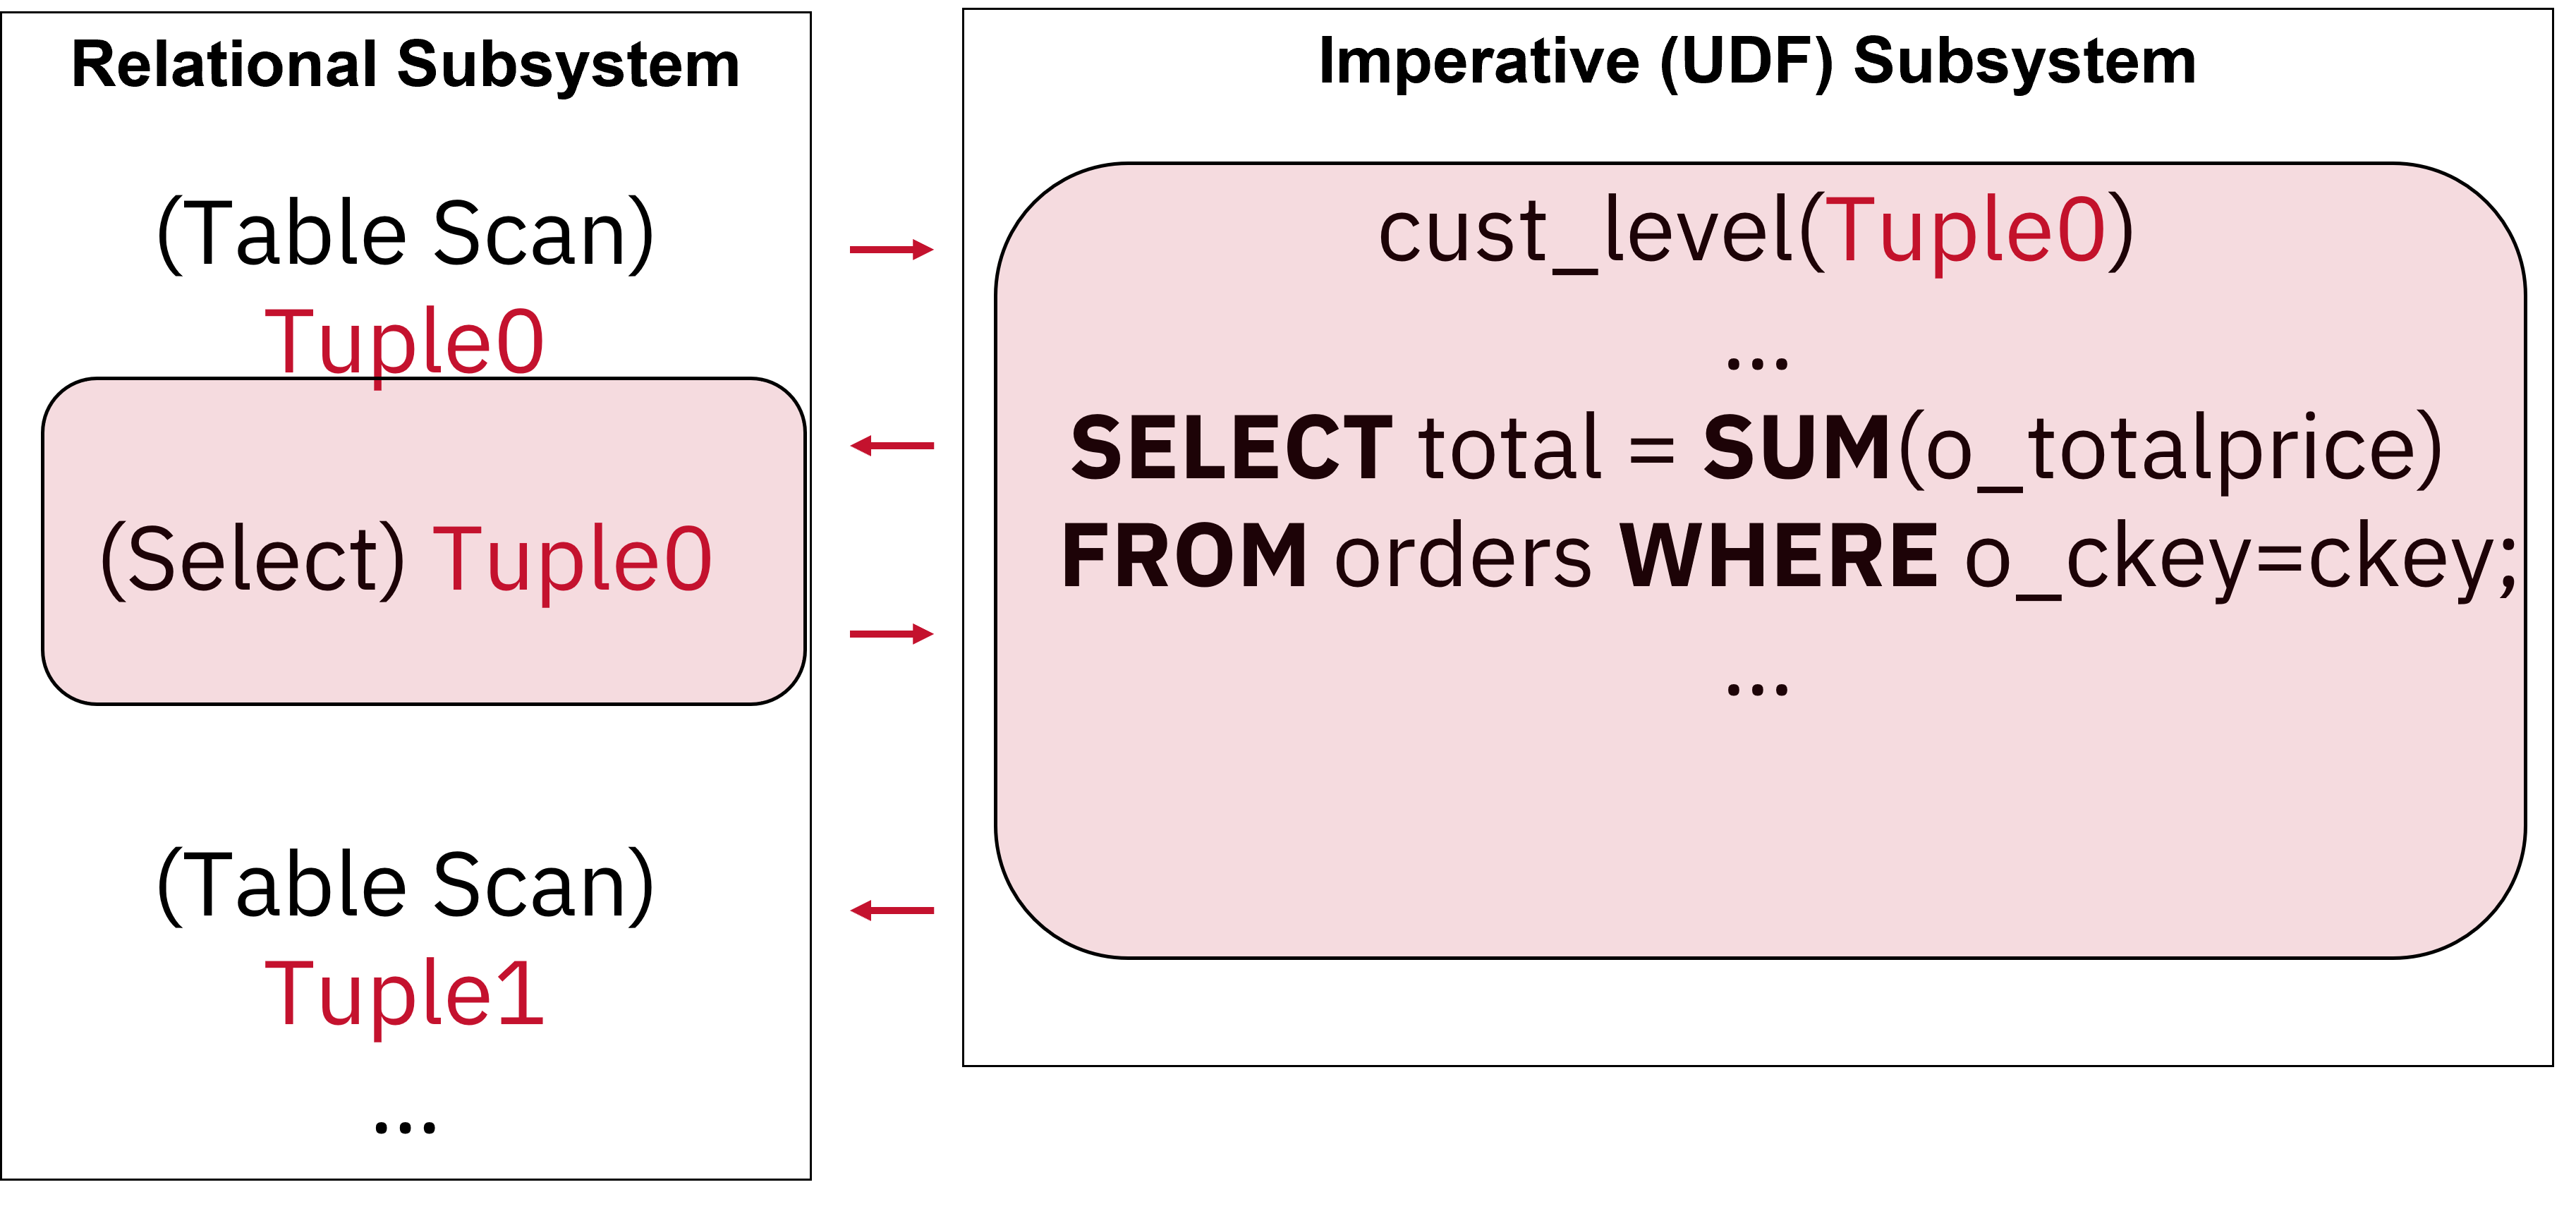
\includegraphics[width=\columnwidth]{img/overhead2.png}
    \caption{
        \textbf{Recursive Context Switching} --
        Most UDFs found in production workloads contain embedded SQL queries. This exacerbates performance issues because the DBMS now context switches between the SQL engine and the imperative engine repeatedly.
    }
    \label{fig:overhead_complex}
\end{figure}

Despite recent advances in compilation techniques, the most successful approaches to addressing the performance limitations of user-defined functions do not involve native compilation. Instead, most of the attention in this space is currently devoted to the technique of UDF inlining. In UDF inlining, a UDF is translated into a relational algebraic expression that can then be embedded directly into the calling SQL query. Inlining a UDF allows the DBMS's existing query optimization component to optimize the logic of an imperative UDF in the same way it optimizes declarative SQL.

Ramachandra et al. implement this technique's archetype in their \textit{Froid} system within Microsoft SQL Server \cite{sqlserver}. Froid executes UDF inlining by first decomposing an individual UDF into distinct \textit{regions} that it then translates into equivalent relational expressions. The Froid framework then relies on SQL Server's \dbCode{APPLY} operator to compose these relational expressions into a single relational expression that encodes the entirety of the UDF's logic \cite{froid}. Gupta et al. extend this work on Froid with their Aggify framework to add support for cursor loops. Aggify realizes its support for cursor loops by translating them to equivalent custom aggregations \cite{aggify}. An example of the inlining technique used by \textit{Froid} is shown in figure~\ref{fig:inlining}.

\begin{figure}[t!]
    \centering
    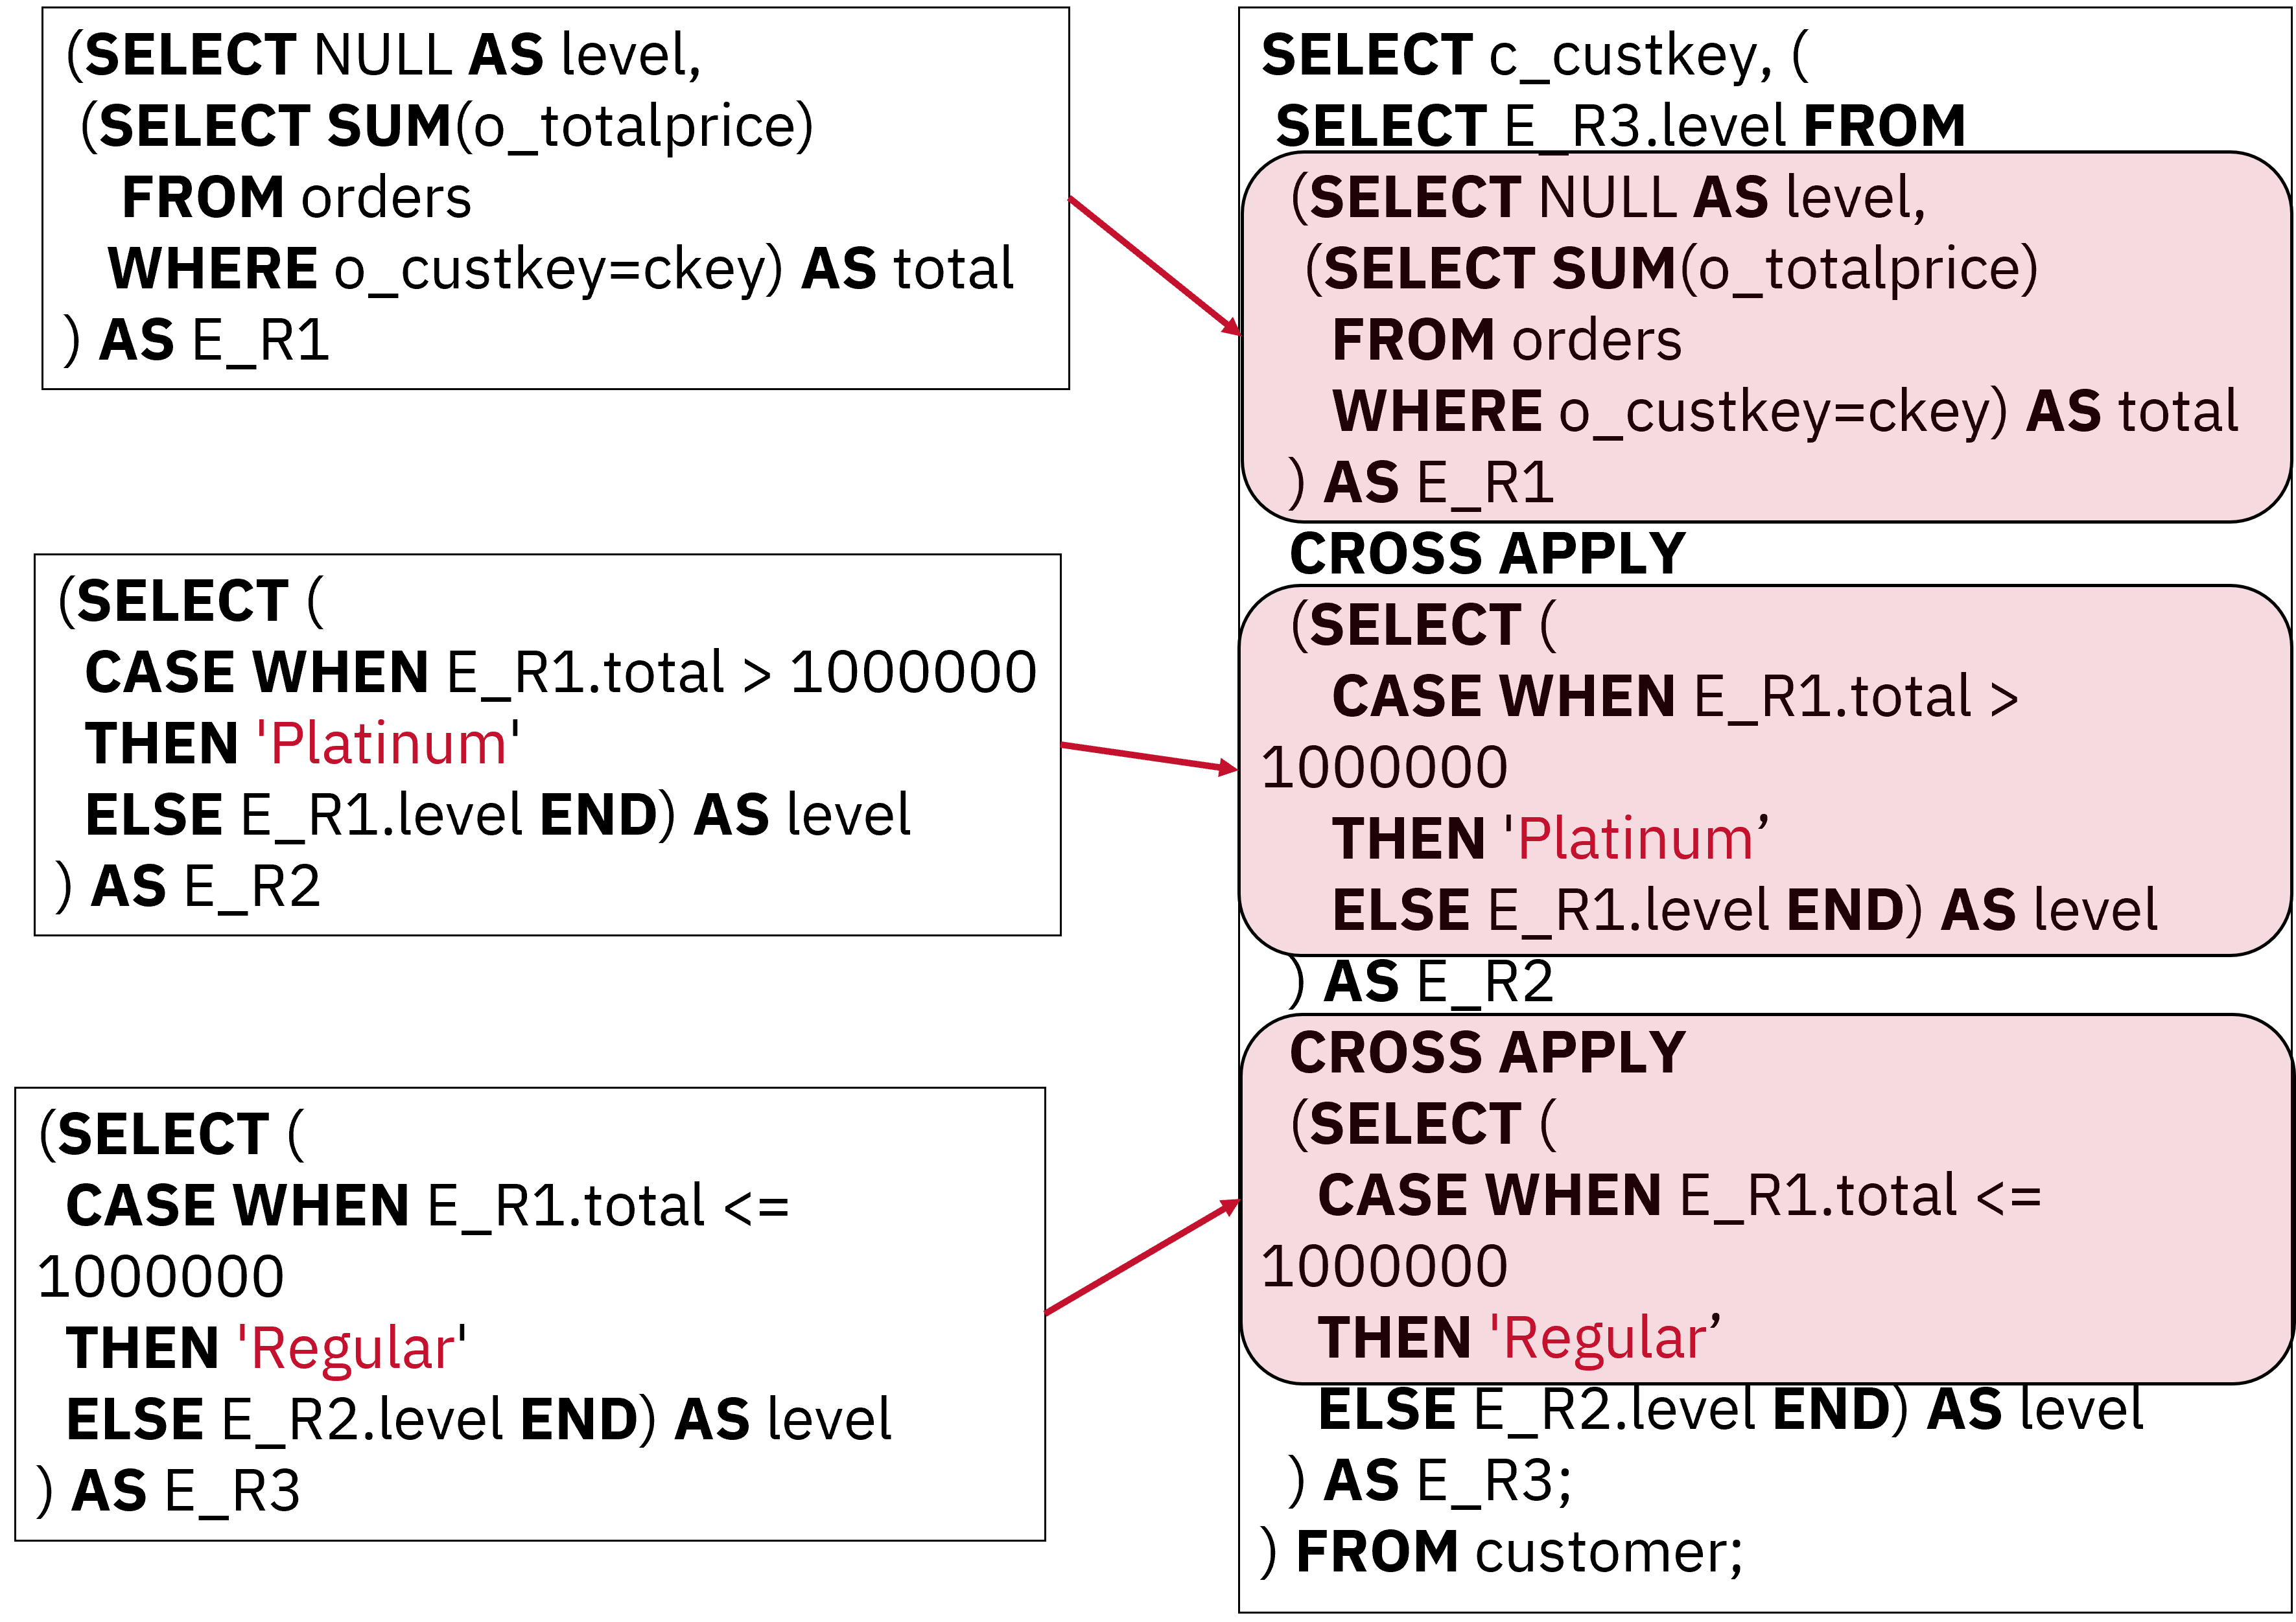
\includegraphics[width=\columnwidth]{img/inlining.png}
    \caption{
        \textbf{UDF Inlining in \textit{Froid}} --
        A simplified example of the UDF-inlining procedure implemented by the \text{Froid} framework in Microsfot SQL Server.
    }
    \label{fig:inlining}
\end{figure}

Duta et al. pursue a distinct approach to UDF inlining in their Apfel framework \cite{apfel}. Where Ramachandra et al. implement Froid as an integrated component of the Microsoft SQL Server DBMS, Duta et al. design their Apfel framework as a standalone system that compiles imperative UDFs written in PL/pgSQL \cite{plpgsql} to standard SQL. Any database system may then process the resulting SQL query in the usual manner. The Apfel framework's defining feature is its use of recursive common table expressions (SQL's \dbCode{WITH RECURSIVE} syntax) to reproduce arbitrary imperative loop logic in SQL.

%% ==================================================================
%% EXECUTION ENGINE
%% ==================================================================

\section{The NoisePage Execution Engine}

The architecture of the NoisePage execution engine is central to the engineering work performed in this project to add support for UDF JIT-compilation. In this section, we describe the internals of the NoisePage execution engine.

We partition the NoisePage execution engine into the following logical layers:

\begin{enumerate}
    \item \textbf{Code Generation}
    \item \textbf{Query Compilation and Execution}
\end{enumerate}

We now describe each of these layers in detail.

\subsection{Physical Query Plan}

The entry point for the NoisePage execution engine is the physical query plan. The physical plan is the query plan produced by the query optimizer. Unlike a logical query plan, the physical plan contains all of the fine-grained query execution decisions that are required to execute the query. For example, the physical query plan explicitly states the algorithms used for \dbSQL{JOIN} operators and the access methods used for table scans.

\subsection{Code Generation}

The code generation layer of the NoisePage execution engine produces a low-level, imperative representation of a query from an input physical query plan. We transform the input query plan through several intermediate stages before emitting the highest-level abstraction that the system is capable of executing - an executable query.

We partition the process of code generation into several logical sub-phases:

\begin{enumerate}
    \item \textit{Pipeline Definition}
    \item \textit{AST Construction}
    \item \textit{Module Generation}
    \item \textit{Executable Query Construction}
\end{enumerate}

We describe each of these sub-phases of code generation below.

\subsubsection{Pipeline Definition}

The \textit{Pipline Definition} phase of code generation translates the input phsyical query plan to the \textit{pipeline} abstraction.

We apply a critical transformation to the query abstraction model at this early stage of processing. The input to code generation is a physical query plan. Internally, this plan is represented as a tree of high-level operators that implement the query. During the initial stages of code generation, however, we break down this abstraction and replace it with the pipeline abstraction.

The pipeline abstraction was originally introduced by Neumann \cite{neumann11} as a means of improving query execution efficiency by exploiting microarchitectural features. Operators from the physical query plan participate in one or more pipelines. A pipeline represents a uni-directional data flow of tuples or tuple batches. Within a pipeline, operators do not materialize tuple (batch) data into cache or memory, which is the primary source of their favorable performance properties.

The procedure for constructing pipelines from the physical query plan proceeds recursively. In the initial traversal of the plan tree, for each plan node we encounter, we perform the following steps
\begin{itemize}
    \item Construct a \textit{translator} for the operator or expression represented by the plan node
    \item In the body of constructor for the translator, recursively prepare the relevant children of the plan node with which this translator is associated
\end{itemize}

A \textit{translator} is a C++ object that is responsible for generating code for a particular query plan operator. We define a unique translator for every physical query plan node. As we descend the plan tree and produce translators for each operator or expression in the physical plan tree, we simultaneously register each translator with one or more pipelines. A translator may appear in multiple pipelines in the event that it represents a materialization point. For instance, consider the translator for the hash join operator. This translator must participate in both the pipeline that produces the tuples utilized on the ``build side'' of the \dbSQL{JOIN} as well as the pipeline that produces tuples utilized on the ``probe side.'' In the NoisePage implementation, the hash join translator constructs a new pipeline with itself as the root to handle this situation.

\subsubsection{AST Construction}

During abstract syntax tree (AST) construction, we translate the pipeline abstraction into an AST for our internal domain-specific language (DSL), \tpl. At this point in code generation, the physical query plan is expressed as a collection of pipelines, each of which is composed of a sequence of translators. The next step in code generation is construction of an AST from the raw pipeline abstraction. This AST subsequently serves as input to the \tpl compiler.

In order to construct an AST from the raw pipeline abstraction, we perform the following steps:

\begin{enumerate}
    \item Declare the top-level structures for the query. The structures are visible to all functions in the compiled query.
    \item Declare top-level functions for the query. Currently, the only top-level functions produced for all queries are those required for query setup and teardown.
    \item Iterate over all pipelines in the query and generate all related pipeline-level code and data. It is at this point that we perform the majority of the work of AST construction. For each pipeline, we iterate over all of the translators defined within it and invoke a set of callback functions in the appropriate order. These functions defer to logic within the translators themselves that emit high-level AST constructs into a common plan.
\end{enumerate}

At the end of AST construction, we now have an AST abstraction that is ready for the \tpl compiler. This AST is organized in much the same way that an AST for a general-purpose programming language is organized. We represent the AST as a collection of data and functions in an approximate control-flow structure that falls short of a proper control-flow graph. During the invocation of the individual translators within each pipeline mentioned above, each translator emits code into the AST at the appropriate point according to the context in which it appears. For example, a translator that appears within pipeline \texttt{Foo} emits the code that implements its functionality into the body of the \texttt{PerformPipelineWork} function for the \texttt{Foo} pipeline. Individual translators are not responsible for emitting the low-level programming constructs that manage control flow (as an example) but rather operate on high-level primitives like table iterators and vector projections.

\subsubsection{TPL Module Generation} 

During \tpl module generation, we transform the AST produced in the previous phase into a \tpl module. A \tpl module contains the bytecode program that implements the query plan.

We implement \tpl compiler as a standalone bytecode compiler. The \tpl compiler performs the following steps to compile the input AST to a \tpl module:

\begin{enumerate}
    \item Parsing: This step is elided in the event that the program is not being compiled from raw TPL source code, which is the case here because we manually constructed the AST for the program during the previous sub-phases of code generation.
    \item Semantic Analysis: The input AST is traversed and checked for logical errors (e.g. type-system violations).
    \item Bytecode Generation: Where the magic happens. The input AST is traversed and translated to a low-level bytecode representation that may be executed directly in a lower layer of the NoisePage execution engine.
    \item Module Generation: A TPL module is constructed that assumes ownership for the raw bytecode produced in the previous step.
\end{enumerate}

There is a one-to-one mapping between code and data defined in the input AST and the code and data that appears in the completed \tpl module. There is no fundamental change to the abstraction that occurs at this stage of code generation. Instead, \tpl module generation represents both an important lowering step (a \tpl module is the fundamental unit of execution for interpreted execution) as well as a unification point between the more general \tpl ecosystem and the NoisePage execution engine. The \tpl compiler can handle both raw \tpl programs in a textual representation as well as a previously-constructed \tpl AST (the intermediary form produced in the previous phase of code generation). Implementing the \tpl ecosystem in a manner that is agnostic of the NoisePage execution engine itself makes the system more amenable to development.

\subsubsection{Executable Query Construction} 

In the final phase of code generation, we transform the \tpl module into an \textit{executable query}. The process of transforming a TPL module into an executable query is straightforward. Each executable query corresponds to a single \tpl module, so we transfer ownership of the module into the executable query. This enforces a relationship in which each query corresponds to exactly one \tpl module.

\subsection{Query Compilation and Execution}

The NoisePage execution engine supports three distinct execution modes:

\begin{itemize}
    \item \texttt{Interpreted}: In interpreted execution, we execute the \tpl bytecode program directly on an interpreter.
    \item \texttt{Compiled}: In compiled execution, we JIT-compile the \tpl bytecode program to native machine code with LLVM \cite{llvm}. We emulate the technique originally proposed by Neumann \cite{neumann11} to accomplish this.
    \item \texttt{Adaptive}: This execution mode attempts to capture the benefits of both of the above execution modes: the low-latency execution of simple queries from \texttt{Interpreted} execution and the high-throughput for complex queries from \texttt{Compiled} execution. This is accomplished by beginning interpreted execution of the query immediately while asynchronously compiling the query in the background. As compilation of query fragments completes, the compiled fragments are dynamically swapped into the running program. This technique was originally proposed by Kohn \cite{kohn18}.
\end{itemize}

In the second logical layer of the NoisePage execution engine, we perform both interpretation of bytecode programs (in \texttt{Interpreted} execution mode) and further compilation of the byetcode program to native machine code (in \texttt{Compiled} execution mode). The interface to each execution mode supported by the execution engine is identical.

As the highest-level of query execution, we perform the same steps regardless of the execution mode:

\begin{enumerate}
    \item Iterate through each function that composes the query and request a C++ function object that implements that function from the fragment's \tpl module. The execution mode is specified in this request to the \tpl module, and it is at this point that the logic of the execution engine diverges based on the execution mode in use.
    \item The \tpl module returns a C++ function object that implements the requested function; we push query processing forward by invoking this function object on the query state and then return to the top of the loop to request the next function from the \tpl module. This process continues until all functions in the query have been executed, at which point the query is complete.
\end{enumerate}

We now examine the internals of each of the available execution modes.

\subsubsection{Interpreted Execution}

In interpreted execution, the function object returned by the \tpl module call wraps an invocation that jumps to the entry point of the NoisePage bytecode interpeter. The implementation of the NoisePage virtual machine is nicely self-contained. The VM implementation in `vm.cpp` may appear daunting at first (the file is nearly 3,000 lines long as of this writing, consisting almost entirely of preprocessor macros) but the actual mechanics of how the VM interprets a query are relatively straightforward.

A single function (\texttt{VM::Interpret()}) implements the core interpreter loop within NoisePage. We implement the \tpl interpreter as a register-based virtual machine (VM). The VM uses indirect threaded interpretation; each bytecode handler's label is statically generated and stored in a predefined location at server compile time. Interpretation of a \tpl program proceeds by reading the first instruction from the bytecode stream, executing it, and returning to the next instruction in the bytecode stream. This process may be influenced by explicit control-flow instructions.

The bytecode handlers defined for the virtual machine are only be simple register and instruction pointer manipulation instructions. The code that contains the logic of these handlers is implemented externally and invoked from the simple instructions in the byetcode stream. This requirement makes code generation to LLVM much simpler in the case that the query is natively compiled.

\subsubsection{Compiled Execution}

We implement the lowest-level stage of query compilation in the NoisePage LLVM engine. The LLVM engine is responsible for JIT-compiling the \tpl bytecode program to native machine code. Once this process is complete, the entirety of the query executes natively on the hardware, without any additional overhead imposed by an interpreter.

Query compilation to machine code takes place in two distinct phases:

\begin{enumerate}
    \item Lowering from the bytecode representation of the \tpl program in the bytecode module to LLVM intermediate representation (IR)
    \item Utilization of the LLVM JIT to compile the LLVM IR to native machine code for the target platform
\end{enumerate}

As the short description above suggests, the first phase is the one we implement ourselves in NoisePage; the majority of the code in the LLVM engine is concerned with this task. Once we lower the \tpl program to LLVM IR, it is a relatively simple matter to utilize the existing LLVM infrastructure to JIT this IR to native code. This is the primary purpose of the LLVM infrastructure, and also why LLVM is a common sight among DBMS execution engines that support compilation to native code.

Once the LLVM IR is compiled to native machine code, we make the native code callable from the DBMS server process itself by:

\begin{enumerate}
    \item Loading the object code for the native machine code into an in-memory buffer
    \item Converting this raw object code into an object file, loading this object file, and linking it to the address space of the DBMS server process
    \item Resolving and caching each of the function definitions in the module. This step is not strictly necessary, but it elides the need to resolve procedures at runtime
\end{enumerate}

Once the native code is loaded and linked to the DBMS process address space, all of the functions it exposes are accessible from regular C++ function calls. The aforementioned use of C++ function objects to wrap these calls unifies the API across calls to both interpreted and compiled functions.

%% ==================================================================
%% UDF COMPILATION
%% ==================================================================

\section{UDF Compilation in NoisePage}

In this section, we describe how we added support for JIT-compilation of user defined functions to the NoisePage DBMS.

TODO

%% ==================================================================
%% EVALUATION
%% ==================================================================

\section{Evaluation}

We now present the results of our evaluation of UDF runtime optimization techniques. We compare our approach to UDF JIT-compilation with several baselines, including interpretation-based UDF execution in PostgreSQL and the inlined SQL queries produced by the \textit{Apfel} framework.

\subsection{Function Call Overhead}

The first aspect of our implementation we intend to evaluate is the overhead imposed by individual function calls. While this does not reflect performance improvements or degregations on production workloads, it does allow us to quickly evaluate the viability of our approach to UDF optimization via JIT compilation.

In order to measure the runtime overhead imposed by an individual function call, we design a simple synthetic benchmark \textit{Call}. This benchmark consists of three queries:

\begin{itemize}
    \item A baseline query that simply performs a sequential scan over a single integer column of a table. This query is shown in listing~\ref{list:udf_call_baseline}. 
    \item A query that invokes the UDF \dbCode{addOne} to increment this integer column by the constant value one. The definition of \dbCode{addOne} is shown in listing~\ref{list:udf_call_functiondef} and the associated invocation is shown in listing~\ref{list:udf_call_function}.
    \item A query that represents a "perfectly-inlined" version of the call to UDf \dbCode{addOne}. In this query, the logic to increment the integer column is completely inlined into the top-level query, eliding the function call entirely. This query is shown in figure~\ref{list:udf_call_inlined}.
\end{itemize}

\begin{listing}
    \begin{minted}[frame=lines]{sql}
SELECT x FROM integers;
    \end{minted}
    \caption{The baseline query for evaluating the overhead of a UDF call.}
    \label{list:udf_call_baseline}
\end{listing}

\begin{listing}
    \begin{minted}[frame=lines]{plpgsql}
CREATE FUNCTION addOne(x INTEGER) 
    RETURNS INTEGER AS $$
BEGIN
    RETURN x + 1;
END
$$ LANGUAGE PLPGSQL;
    \end{minted}
    \caption{The definition of UDF \dbCode{addOne}.}
    \label{list:udf_call_functiondef}
\end{listing}

\begin{listing}
    \begin{minted}[frame=lines]{sql}
SELECT x, addOne(x) FROM integers;
    \end{minted}
    \caption{The inlined query for evaluating the overhead of a UDF call.}
    \label{list:udf_call_function}
\end{listing}

\begin{listing}
    \begin{minted}[frame=lines]{sql}
SELECT x, x + 1 FROM integers;
    \end{minted}
    \caption{The inlined query for evaluating the overhead of a UDF call.}
    \label{list:udf_call_inlined}
\end{listing}

We run this performance benchmark on two systems: PostgreSQL 12 and NoisePage. Here, PostgreSQL serves as a baseline against which we compare our implementation. PostgreSQL implements UDF execution in a manner that incurs significant context-switching overhead \cite{apfel}. As a consequence of this, we expect to observe high function-call overhead in PostgreSQL. In contrast, the benchmark run on NoisePage uses our approach to UDF JIT-compilation that should avoid context switching overhead by virtue of the fact that all of the logic is expressed as a single program in our internal DSL. 

The results of this benchmark are shown in figure~\ref{fig:bench_pg_call} and figure~\ref{fig:bench_np_call}. The results demonstrate the expected trend: UDF execution in PostgreSQL is slower in absolute terms than UDF execution in NosiePage. More importantly, as the size of the table grows, the overall query runtime for PostgreSQL scales much more poorly that it does for NoisePage. This indicates that our implementation of UDF JIT-compilation does not incur large function call overhead, relative to the "optimal" inlined version of the query.

\begin{figure}[t!]
    \centering
    
\includegraphics[width=\columnwidth]{plots/pg_call_legend.pdf}
    \\
    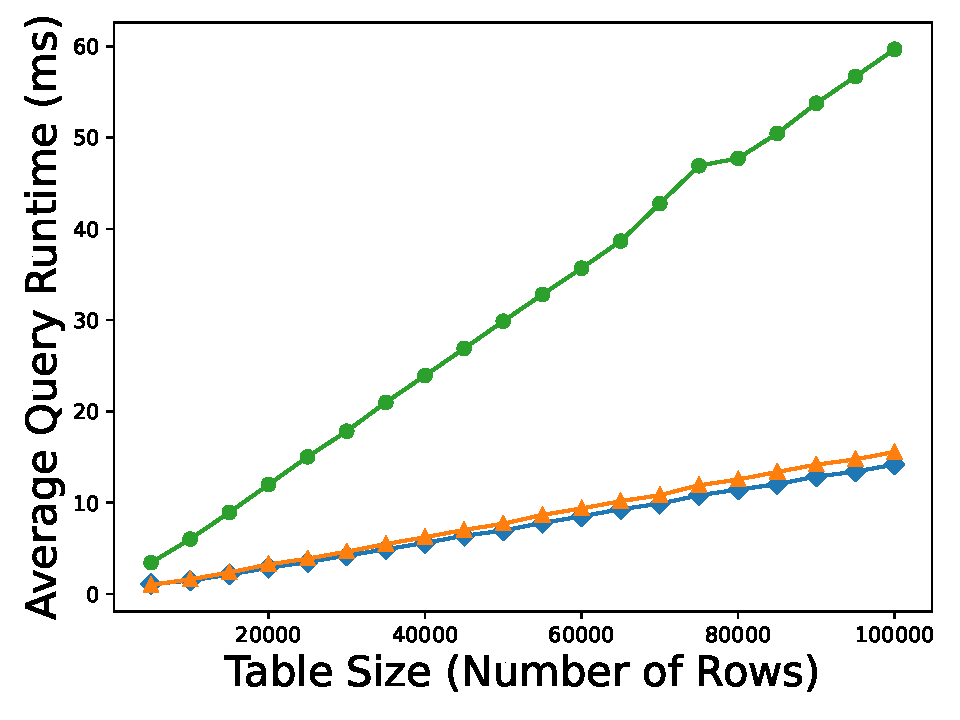
\includegraphics[width=\columnwidth]{plots/pg_call.pdf}
    \caption{
        \textbf{Function Call Overhead (PostgreSQL)} --
        Comparison among baseline query, inlined column increment, and column increment with a function call to UDF \dbCode{addOne} in PostgreSQL.
    }
    \label{fig:bench_pg_call}
\end{figure}

\begin{figure}[t!]
    \centering
    
\includegraphics[width=\columnwidth]{plots/np_call_legend.pdf}
    \\
    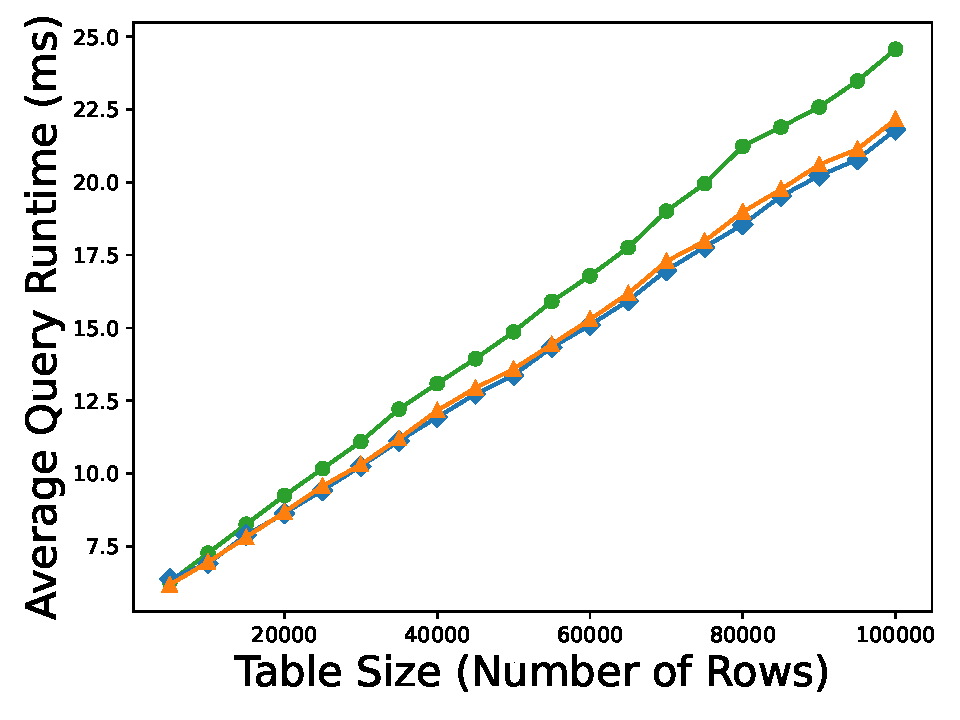
\includegraphics[width=\columnwidth]{plots/np_call.pdf}
    \caption{
        \textbf{Function Call Overhead (NoisePage)} --
        Comparison among baseline query, inlined column increment, and column increment with a function call to UDF \dbCode{addOne} in NoisePage.
    }
    \label{fig:bench_np_call}
\end{figure}

\subsection{Lighweight Loops}

We construct a second benchmark, \textit{Loop}, to evaluate the viability of our approach to UDF JIT-compilation against the PostgreSQL baseline. In this benchmark, we evaluate the total runtime required for the UDF execution engine to execute a tight loop for a specified number of iterations. Like the previous benchmark, this benchmark does not serve as an indicator of performance on production workloads, but rather demonstrates the potential of our approach to remove software overheads via JIT-compilation of functions.

The definition of the \dbCode{busyLoop} function is provided in listing~\ref{list:udf_loop}. This function is invoked with arguments ranging from 10-100,000,000 specifying the number of iterations of the loop executed within the function's body. The results of the benchmark are shown in figure~\ref{fig:bench_loop}. We see that as the number of iterations grows by a factor of 10, increasing from 10,000,000 to 100,000,000, the total query runtime on PostgreSQL explodes as a result of the relatively-high overhead of individual iterations. In contrast, the growth in runtime for NoisePage is much more modest, suggesting that our approach to UDF JIT-compilation elides much of the overhead imposed by interpreter-based systems like PostgreSQL.

\begin{listing}
    \begin{minted}[frame=lines]{plpgsql}
CREATE FUNCTION busyLoop(x INTEGER) 
    RETURNS INTEGER AS $$
DECLARE
    c INTEGER := 0;
BEGIN
    WHILE c < x LOOP;
        c = c + 1;
    END LOOP;
    RETURN c;
END
$$ LANGUAGE PLPGSQL;
    \end{minted}
    \caption{The definition of UDF \dbCode{busyLoop}.}
    \label{list:udf_loop}
\end{listing}

\begin{figure}[t!]
    \centering
    
\includegraphics[width=\columnwidth]{plots/loop_legend.pdf}
    \\
    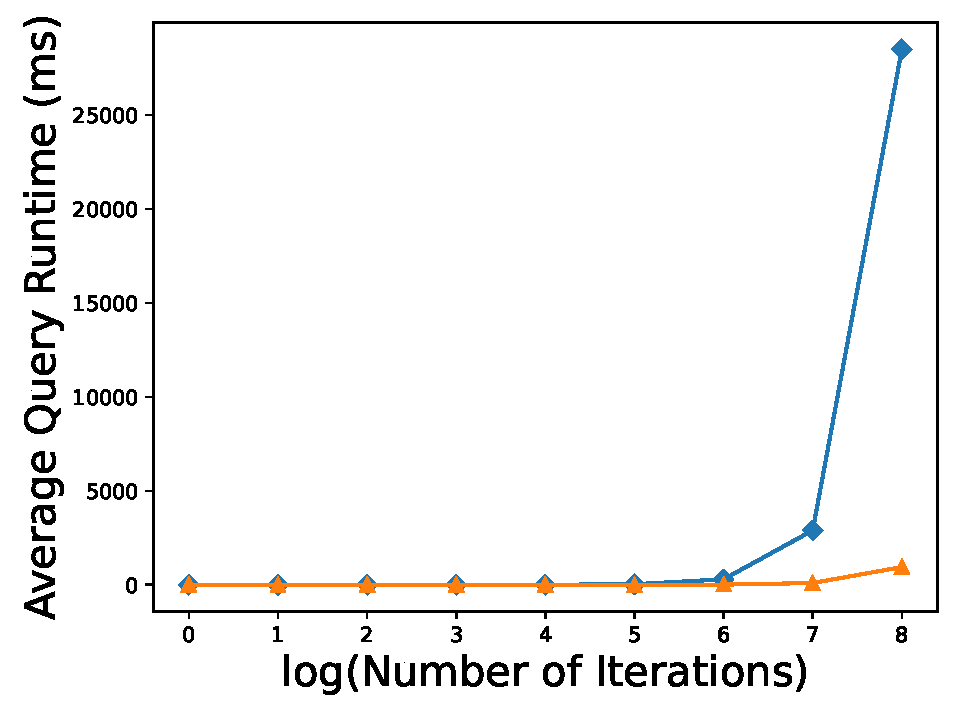
\includegraphics[width=\columnwidth]{plots/loop.pdf}
    \caption{
        \textbf{Function Call Scalability} --
        Comparison of the runtime required by PostgreSQL and NoisePage to execute the UDF \dbCode{busyLoop} for a specified number of iterations.
    }
    \label{fig:bench_loop}
\end{figure}

Finally, we perform an initial evaluation on a selected functions from the SQL ProcBench \cite{procbench} benchmark. The performance evaluation is performed on the NoisePage system. Results from running this benchmark against PostgreSQL 12 are also included to provide a point of comparison. We note that, unlike the previous synthetic benchmarks, this benchmark reflects the complete end-to-end performance characteristics of the tested system, rather than the performance characteristics of the UDF execution subsystem in isolation. Results of this benchmark are shown in figure~\ref{fig:bench_procbench}.

\begin{figure}[t!]
    \centering
    
\includegraphics[width=\columnwidth]{plots/procbench_legend.pdf}
    \\
    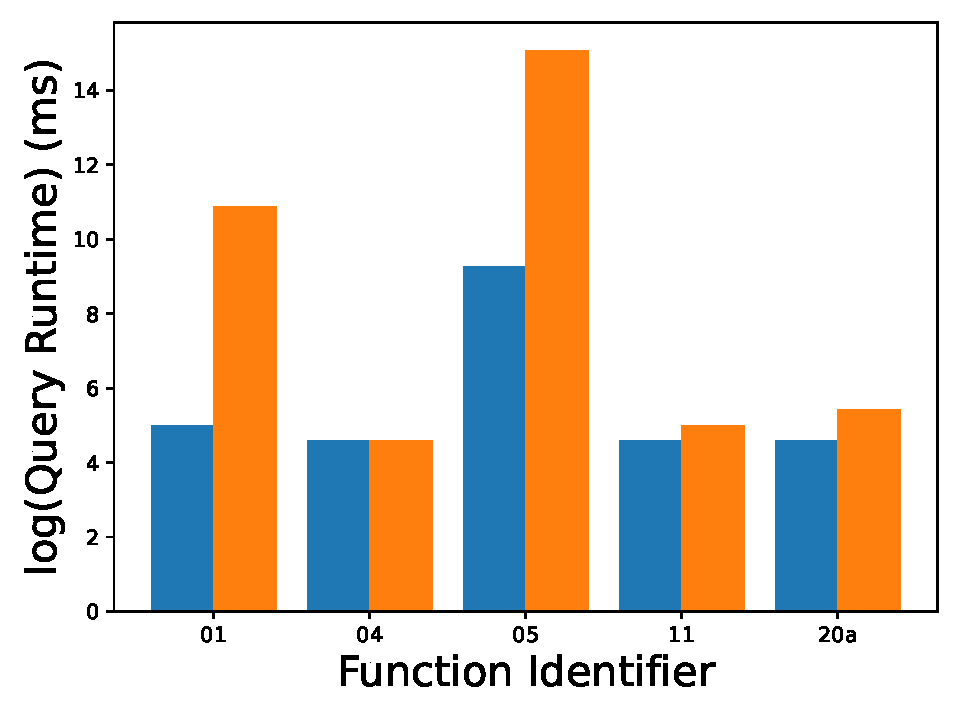
\includegraphics[width=\columnwidth]{plots/procbench.pdf}
    \caption{
        \textbf{End-to-End Benchmark Performance} --
        Comparison of query runtime on PostgreSQL and NoisePage during execution of select functions from the SQL ProcBench benchmark.
    }
    \label{fig:bench_procbench}
\end{figure}

Unlike the previous two benchmarks, the results of this benchmark are far from inspiring. NoisePage achieves runtimes similar to PostgreSQL for several of the functions (function identifiers \dbCode{04}, \dbCode{11}, and \dbCode{20a}), but far underperforms PostgreSQL on the remaining functions (function identifiers \dbCode{01} and \dbCode{05}). The distinction between these two sets of functions is that functions in the former group does not interact heavily with the NoisePage storage subsystem, while functions in the latter group do. As a specific example, the definition of the UDF with function identifier \dbCode{05} is shown in listing~\ref{list:udf_procbench_05}. The logic in this function is not complex, but it does involve two aggregations over the result of a three-way \dbCode{JOIN} on three relatively-large tables, implying that most of the work for this query occurs in the storage subsystem as tables are scanned and the \dbCode{JOIN} predicates are applied. The NoisePage storage subsystem has several design deficiencies that render this bottleneck unavoidable.

NoisePage's poor performance on these benchmark functions does not directly influence our ability to complete our evaluation. From the beginning of this project, we have planned to conduct our evaluation within the context of a single research platform in order to neutralize precisely these types of differences among database systems. However, it might preclude our ability to produce results suitable for publication.

\begin{listing}
    \begin{minted}[frame=lines]{plpgsql}
CREATE OR REPLACE FUNCTION morningToEveRatio(dep INT) 
    RETURNS INT AS $$
DECLARE
    morningSale INT;
    eveningSale INT;
    totalSale INT;
BEGIN
    morningSale := (SELECT COUNT(*)
        FROM web_sales, time_dim, customer_demographics
        WHERE ws_sold_time_sk = t_time_sk 
            AND ws_bill_customer_sk = cd_demo_sk
            AND t_hour >= 8 AND t_hour <= 9
            AND cd_dep_count = dep);

    eveningSale := (SELECT COUNT(*)
        FROM web_sales, time_dim, customer_demographics 
        WHERE ws_sold_time_sk = t_time_sk 
            AND ws_bill_customer_sk = cd_demo_sk
            AND t_hour >= 19 AND t_hour <= 20
            AND cd_dep_count = dep);

    totalSale := morningSale + eveningSale;
    RETURN totalSale;
END; 
$$ LANGUAGE PLPGSQL;
    \end{minted}
    \caption{The definition of ProcBench UDF \dbCode{05}.}
    \label{list:udf_procbench_05}
\end{listing}

%% ==================================================================
%% FUTURE WORK
%% ==================================================================

\section{Future Work}

While we completed our intended evaluation in this project, many promising directions for future work remain. 

%% ==================================================================
%% CONCLUSION
%% ==================================================================

\section{Conclusion}

TODO

%% ==================================================================
%% ACKNOWLEDGEMENTS
%% ==================================================================

\section{Acknowledgements}

I would like to thank Karthik Ramachandra from Microsoft for providing insights on the \textit{Froid} framework and its approach to UDF-inlining. I would also like to thank Surabhi Gupta for her work on the SQL ProcBench benchmark. I would also like to thank Torsten Grust and Denis Hirn from the University of Tubingen for providing insights on their \textit{Apfel} framework and providing the means to inline selected queries for our evaluation. I would like to thank my Capstone advisor Andrew Pavlo for his consistent feedback and enthusiasm for this project. Finally, I would like to thank all of my colleagues in the Carnegie Mellon Database Group for constantly inspiring me to strive for database-greatness.

%% ==================================================================
%% BIBLIOGRAPHY
%% ==================================================================

% NOTE: Had to add this mysterious command to compile...
\newcommand{\newblock}{}

\clearpage
\bibliographystyle{abbrv}
\bibliography{final}

\end{document}